% Provenance (never printed): see sources/outline_sources.md (Year 3:
% facies analysis, depositional models, Walther's law, well logs). Brief:
% sources/book5/BRIEFS.md, ch. 17. Curves from figdata/bachelor-3/well_logs.py
% (unit tops from figdata/shared/region.py). Exercise and problem values in
% the Book 5 scratch calculator calc/ch17.py. The well Varden-2, its logs and
% the channel architecture of its sandstone are invented.
\chapter{Faciesmodellen}\label{ch:b3:facies-models}

Een kern uit een put van een kilometer diep: een meter grof zand met
kruislaminatie op een scherpe basis, opwaarts fijner wordend tot silt met de
sporen van wortels, daarna weer zand op een andere scherpe basis. De geoloog leest een rivier
die over zijn vlakte kronkelde, hoewel er nu geen rivier meer loopt. De lezing
steunt op twee hulpmiddelen: een reeks modellen, elk een samenvatting van vele moderne en
oude voorbeelden van één milieu, en een wet die een verticale
opeenvolging van lagen omzet in een kaart van naburige milieus.

\begin{recall}
Sedimentaire facies, afzettingsmilieu, bodemvormen, kruislaminatie,
delta's van de drie soorten, troebelingsstromen, turbidieten en gradatielagen
staan in Boek~3, in het hoofdstuk over klastische sedimenten en hun
milieus; de karbonaatfabriek, riffen en karbonaatplatforms in het
hoofdstuk over karbonaat-, kiezelige en evaporietsedimenten; de boorstaat en
de correlatie van logs in het hoofdstuk over doorsnedes. Porositeit en
permeabiliteit staan in de schoolboeken. \omterm{def:b3:sequence-stratigraphy:parasequence}{Parasequenties}, overstromingsvlakken en
\omterm{def:b3:sequence-stratigraphy:tract}{systeemtracten} staan in Hoofdstuk~\ref{ch:b3:sequence-stratigraphy}. Golven op
diep water, waarvan de beweging met de diepte afneemt, staan in de natuurkundeboeken.
\end{recall}

\section{Facies, opeenvolgingen en de wet van Walther}\label{sec:b3:facies-models:walther}

Een sedimentaire facies wordt beschreven aan de hand van wat zichtbaar is in
een kern of een klif: korrelgrootte, sortering, structuren, fossielen, kleur. Een enkele facies is
zelden diagnostisch: kruisgelaagd zand ontstaat in rivieren, op stranden, in
getijdegeulen en in woestijnen. Wat een milieu identificeert, is het gezelschap waarin een
facies voorkomt en de volgorde waarin facies op elkaar volgen.

\begin{definition}[Faciesassociatie en faciesopeenvolging]\label{def:b3:facies-models:association}
Een \emph{faciesassociatie}\index{faciesassociatie} is een groep facies die
samen voorkomt en in één milieu is afgezet, zoals
geulzand, oeverslib en overstromingsklei met wortels. Een \emph{faciesopeenvolging}\index{faciesopeenvolging}
is een verticale reeks facies waarin
een eigenschap geleidelijk opwaarts verandert; in een \emph{opwaarts fijner
wordende opeenvolging}\index{opwaarts fijner wordende opeenvolging} neemt de korrelgrootte naar boven toe af,
in een \emph{opwaarts grover wordende opeenvolging}\index{opwaarts grover wordende opeenvolging}
neemt zij toe.
\end{definition}

\begin{definition}[Faciesmodel]\label{def:b3:facies-models:model}
Een \emph{faciesmodel}\index{faciesmodel} is een algemene samenvatting van een
afzettingsmilieu, gedestilleerd uit vele moderne en oude voorbeelden: de
facies die het voortbrengt, hun geometrie, hun laterale verbanden en de
opeenvolgingen die zij opbouwen. Het dient als norm om een nieuw voorbeeld mee,
te vergelijken, als leidraad voor verder onderzoek, als voorspeller in nieuwe situaties en als basis voor
de interpretatie van het milieu.
\end{definition}

De brug tussen het laterale en het verticale is een wet. Naburige milieus
liggen op elk moment naast elkaar: het strand naast de \omterm{def:b3:facies-models:shoreface}{onderwateroever}, de
\omterm{def:b3:facies-models:shoreface}{onderwateroever} naast de klei van de diepere zee. Wanneer de kustlijn
verschuift, komt elk milieu over zijn buur te liggen.

\begin{theorem}[Wet van Walther]\label{thm:b3:facies-models:walther}
In een concordante opeenvolging, zonder een aanzienlijke onderbreking in de afzetting of een
erosievlak, zijn facies die direct boven elkaar liggen afgezet in
milieus die op dat moment naast elkaar lagen.
\end{theorem}

\begin{proof}
Beschouw gordels van milieus, elk een strook evenwijdig aan de kustlijn, die
samen over het bekken migreren terwijl de bodem zakt of het zeeniveau
stijgt. Op een vaste plaats schuiven de gordels één voor één langs, in de volgorde
waarin zij naast elkaar liggen, en elk laat zijn afzetting achter bovenop de
afzetting van de gordel die eraan voorafging. Als de afzetting continu is, is
de verticale volgorde van de afzettingen dus de laterale volgorde van de
gordels. Een onderbreking of een erosievlak doorbreekt het argument: de gordels die
in de tussentijd passeerden, lieten niets achter, of hun afzettingen zijn weggeslagen, en facies uit
niet-aangrenzende milieus komen met elkaar in contact.
\end{proof}

\begin{omfigure}
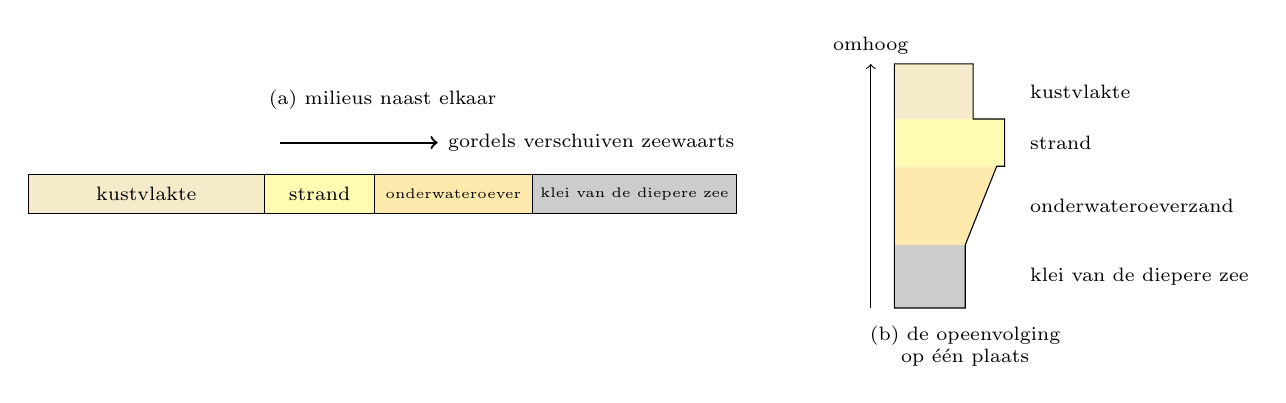
\begin{tikzpicture}[font=\scriptsize, x=1cm, y=1cm]
% environments side by side, with a shoreline that moves seaward
\fill[yellow!35!brown!25] (0,0) rectangle (3,0.5);
\fill[yellow!30] (3,0) rectangle (4.4,0.5);
\fill[yellow!50!orange!30] (4.4,0) rectangle (6.4,0.5);
\fill[black!20] (6.4,0) rectangle (9,0.5);
\draw (0,0) rectangle (9,0.5);
\foreach \x in {3,4.4,6.4} {\draw (\x,0) -- (\x,0.5);}
\node at (1.5,0.25) {kustvlakte};
\node at (3.7,0.25) {strand};
\node[font=\tiny] at (5.4,0.25) {onderwateroever};
\node[font=\tiny] at (7.7,0.25) {klei van de diepere zee};
\draw[->, thick] (3.2,0.9) -- (5.2,0.9) node[right] {gordels verschuiven zeewaarts};
\node[anchor=south] at (4.5,1.2) {(a) milieus naast elkaar};
% vertical succession at a place
\begin{scope}[xshift=11cm, yshift=-1.2cm]
\fill[black!20] (0,0) rectangle (0.9,0.8);
\fill[yellow!50!orange!30] (0,0.8) -- (0.9,0.8) -- (1.3,1.8) -- (0,1.8) -- cycle;
\fill[yellow!30] (0,1.8) rectangle (1.4,2.4);
\fill[yellow!35!brown!25] (0,2.4) rectangle (1.0,3.1);
\draw (0,0) -- (0.9,0) -- (0.9,0.8) -- (1.3,1.8) -- (1.4,1.8) -- (1.4,2.4) -- (1.0,2.4) -- (1.0,3.1) -- (0,3.1) -- cycle;
\node[anchor=west] at (1.6,0.4) {klei van de diepere zee};
\node[anchor=west] at (1.6,1.3) {onderwateroeverzand};
\node[anchor=west] at (1.6,2.1) {strand};
\node[anchor=west] at (1.6,2.75) {kustvlakte};
\draw[->] (-0.3,0) -- (-0.3,3.1) node[above] {omhoog};
\node[anchor=north, align=center] at (0.9,-0.1) {(b) de opeenvolging\\ op één plaats};
\end{scope}
\end{tikzpicture}

\par\smallskip{\small De wet van Walther. (a) Milieus liggen naast elkaar langs
een profiel; (b) terwijl de gordels zeewaarts verschuiven, krijgt één plaats eerst offshore-modder,
daarna onderwateroeverzand, strandzand en afzettingen van de kustvlakte: een
\omterm{def:b3:facies-models:association}{opwaarts grover wordende opeenvolging} in de volgorde van de gordels (breedte in de log
betekent grover korrelmateriaal).}\label{fig:b3:facies-models:walther}
\end{omfigure}

De wet werkt in beide richtingen. Een regressie stapelt de gordels in hun zeewaartse
volgorde opwaarts, een transgressie in omgekeerde volgorde; en een verticale opeenvolging die in
een kern wordt gelezen, geeft de kaart van de naburige milieus op dat moment. Ze faalt
precies daar waar in Hoofdstuk~\ref{ch:b3:sequence-stratigraphy} de sleutelvlakken liggen:
over een \omterm{def:b3:sequence-stratigraphy:sequence}{sequentiegrens}, waar blootstelling en erosie rivierzand op shelfmodder brengen, en
over een \omterm{def:b3:sequence-stratigraphy:parasequence}{overstromingsvlak}, waar offshore-modder direct op
de kustvlakte ligt.

\section{Rivieren}\label{sec:b3:facies-models:rivers}

\begin{definition}[Verwilderde en meanderende rivieren]\label{def:b3:facies-models:rivers}
Een \emph{verwilderde rivier}\index{verwilderde rivier} stroomt in meerdere ondiepe
geulen die zich om bars splitsen en weer samenkomen, op een steile vlakte met veel
grof materiaal en wisselend debiet. Een \emph{meanderende rivier}\index{meanderende rivier}
stroomt in één kronkelende geul op een flauwere vlakte en voert meer
fijn sediment mee; ze migreert door de buitenoever van elke bocht te eroderen en
op de binnenoever af te zetten. De afzetting op de binnenoever is een \emph{kronkelwaard}\index{kronkelwaard}.
\emph{Avulsie}\index{avulsie} is het verlaten van een geul voor een nieuw
traject over de overstromingsvlakte, meestal nadat een overstroming
een dijk doorbreekt.
\end{definition}

Een \omterm{def:b3:facies-models:rivers}{kronkelwaard} groeit zijwaarts terwijl de bocht migreert, zodat hij op elke plaats
de dwarsdoorsnede van de geul van onder naar boven vastlegt: een lag van het
grofste puin op een erosiebasis, kruisgelaagd zand van de duinen in de diepe
geul, fijner zand met rimpels van de ondiepe top van de bar, en daarna de
silt en modder van de overstromingsvlakte met wortels en bodems. Volgens de wet van Walther heeft deze
\omterm{def:b3:facies-models:association}{opwaarts fijner wordende opeenvolging}, enkele meters dik, de dikte van de
diepte van de geul. Een \omterm{def:b3:facies-models:rivers}{verwilderde rivier} laat gestapelde lagen kruisgelaagd zand
en grind achter met weinig modder, waarvan de korrelgrootte opwaarts nauwelijks verandert; het fijne
materiaal wordt weggevoerd. \omterm{def:b3:facies-models:rivers}{Avulsie} verplaatst de geulgordel over de vlakte, zodat
geullichamen willekeurig stapelen tussen modder van de overstromingsvlakte, gescheiden door scherpe
erosiebases.

\begin{omfigure}
\begin{tikzpicture}[font=\scriptsize, x=1cm, y=1cm]
% (a) braided plan
\begin{scope}
\fill[yellow!35!brown!20] (0,0) rectangle (4.6,2.4);
\draw[omDef!60, line width=1.6pt] (0,1.2) .. controls (0.8,1.6) and (1.4,0.6) .. (2.3,1.0) .. controls (3.0,1.3) and (3.6,0.7) .. (4.6,1.0);
\draw[omDef!60, line width=1.6pt] (0,1.2) .. controls (0.8,0.8) and (1.6,1.9) .. (2.4,1.6) .. controls (3.2,1.3) and (3.8,1.9) .. (4.6,1.6);
\draw[omDef!60, line width=1.2pt] (1.2,1.25) .. controls (1.8,1.5) and (2.6,1.2) .. (3.3,1.35);
\fill[yellow!45] (1.5,1.15) ellipse (0.35 and 0.12);
\fill[yellow!45] (3.0,1.25) ellipse (0.4 and 0.12);
\node[anchor=south] at (2.3,2.45) {(a) verwilderd};
\end{scope}
% (b) meandering plan
\begin{scope}[xshift=5.4cm]
\fill[green!30!black!12] (0,0) rectangle (4.6,2.4);
\draw[omDef!60, line width=2pt] (0,1.2) .. controls (0.6,2.2) and (1.4,2.2) .. (1.6,1.2) .. controls (1.8,0.2) and (2.8,0.2) .. (3.0,1.2) .. controls (3.2,2.2) and (4.0,2.2) .. (4.6,1.2);
\fill[yellow!45] (0.8,1.45) ellipse (0.3 and 0.2);
\fill[yellow!45] (2.3,0.95) ellipse (0.3 and 0.2);
\fill[yellow!45] (3.8,1.45) ellipse (0.3 and 0.2);
\node at (2.3,0.95) {pb};
\draw[omDef!40, line width=1pt, densely dashed] (0.4,0.2) .. controls (1.0,0.7) and (1.6,0.4) .. (2.0,0.1);
\node[anchor=west, font=\tiny] at (2.6,2.15) {overstromingsvlakte};
\node[anchor=south] at (2.3,2.45) {(b) meanderend};
\end{scope}
% logs
\begin{scope}[xshift=10.8cm]
\fill[yellow!45] (0,0) -- (1.2,0) -- (1.2,2.0) -- (0,2.0) -- cycle;
\draw (0,0) -- (1.2,0) -- (1.15,0.6) -- (1.2,0.65) -- (1.1,1.3) -- (1.2,1.35) -- (1.15,2.0) -- (0,2.0) -- cycle;
\node[anchor=north] at (0.6,-0.05) {verwilderd};
\end{scope}
\begin{scope}[xshift=12.6cm]
\fill[yellow!45] (0,0) -- (1.2,0) -- (1.1,0.9) -- (0.45,1.6) -- (0,1.6) -- cycle;
\fill[green!30!black!15] (0,1.6) rectangle (0.3,2.2);
\draw (0,0) -- (1.2,0) -- (1.1,0.9) -- (0.45,1.6) -- (0.3,1.6) -- (0.3,2.2) -- (0,2.2) -- cycle;
\draw[decorate, decoration={snake, amplitude=0.4mm, segment length=1.5mm}] (0,0) -- (1.2,0);
\node[anchor=north] at (0.6,-0.05) {kronkelwaard};
\node[anchor=west, font=\tiny] at (0.35,1.9) {wortels};
\end{scope}
\end{tikzpicture}

\par\smallskip{\small (a) Een \omterm{def:b3:facies-models:rivers}{verwilderde rivier}: meerdere geulen rond bars van
zand en grind. (b) Een \omterm{def:b3:facies-models:rivers}{meanderende rivier}: één kronkelende geul, \omterm{def:b3:facies-models:rivers}{kronkelwaarden} (pb)
op de binnenoevers, een verlaten traject (gestippeld) achtergelaten door \omterm{def:b3:facies-models:rivers}{avulsie}. Rechts:
korrelgroottelogs van de afzettingen (breedte betekent grover materiaal): gestapelde zandlagen
met weinig verandering naar boven voor de \omterm{def:b3:facies-models:rivers}{verwilderde rivier}, en een scherp begrensde, \omterm{def:b3:facies-models:association}{opwaarts fijner wordende
opeenvolging} afgedekt door bewortelde modder van de overstromingsvlakte voor de \omterm{def:b3:facies-models:rivers}{kronkelwaard}.
}\label{fig:b3:facies-models:rivers}
\end{omfigure}

\section{Kustlijnen, delta's en shelven}\label{sec:b3:facies-models:shelves}

De delta's uit Boek~3, gedomineerd door rivieren, golven of getijden, bouwen zich allemaal
op hetzelfde mechanisme: de monding zet haar vracht af waar de
stroming vertraagt, en het deltafront schuift over zijn eigen prodeltamodder vooruit. Een
prograderend deltafront of \omterm{def:b3:facies-models:shoreface}{onderwateroever} laat volgens de wet van Walther een
\omterm{def:b3:facies-models:association}{opwaarts grover wordende opeenvolging} achter: offshore-modder, afwisselend modder en stormzand,
onderwateroeverzand, strand. Elke \omterm{def:b3:sequence-stratigraphy:parasequence}{parasequentie} uit het vorige hoofdstuk is zo'n
opeenvolging.

\begin{definition}[Onderwateroever en golfbases]\label{def:b3:facies-models:shoreface}
De \emph{onderwateroever}\index{onderwateroever} is de hellende zone zeewaarts van het
strand waar golven voortdurend de zeebodem omwerken. De basis ervan is de
\emph{golfbasis bij mooi weer}\index{golfbasis bij mooi weer}, de diepte waaronder
gewone golven het bodemsediment niet meer in beweging brengen. De \emph{golfbasis bij storm}\index{golfbasis bij storm}
is de diepere grens die door stormgolven wordt bereikt;
tussen die twee bezinkt modder bij rustig weer en wordt omgewerkt tot zandlagen
tijdens stormen. Onder de golfbasis bij storm wordt de bodem niet door golven verstoord.
\end{definition}

\begin{omfigure}
\begin{tikzpicture}[font=\scriptsize, x=1cm, y=1.6cm]
\fill[omSea!60] (0,2.2) -- (13,2.2) -- (13,0.2) -- (5.5,0.9) -- (2.0,1.9) -- (0.6,2.2) -- cycle;
\fill[yellow!40] (0,2.4) -- (0.6,2.2) -- (2.0,1.9) -- (5.5,0.9) -- (5.5,0.0) -- (0,0.0) -- cycle;
\fill[black!18] (5.5,0.9) -- (13,0.2) -- (13,0) -- (5.5,0) -- cycle;
\draw[thick] (0,2.4) -- (0.6,2.2) -- (2.0,1.9) -- (5.5,0.9) -- (13,0.2);
\draw[omDef] (0,2.2) -- (13,2.2);
\draw[omDef, densely dashed] (1.6,1.97) -- (13,1.97);
\draw[omDef, densely dashed] (5.5,0.9) -- (13,0.9);
\node[omDef, anchor=north west] at (9.3,1.95) {golfbasis bij mooi weer};
\node[omDef, anchor=north west] at (9.3,0.88) {golfbasis bij storm};
\node[anchor=south] at (0.5,2.42) {strand};
\node at (1.8,1.35) {onderwateroever};
\node at (4.3,0.45) {overgang naar de open zee};
\node at (9.0,0.15) {modder op open zee};
\node[align=center] at (7.4,1.45) {stormzandlagen,\\ hummocky kruisgelaagdheid};
\end{tikzpicture}

\par\smallskip{\small Een golfgedomineerd kustprofiel (schematisch, verticale
schaal sterk overdreven). Boven de \omterm{def:b3:facies-models:shoreface}{golfbasis bij mooi weer} wordt het zand van de
\omterm{def:b3:facies-models:shoreface}{onderwateroever} elke dag omgewerkt; tussen de twee golfbases wisselt modder af met
door storm afgezette zandlagen; onder de \omterm{def:b3:facies-models:shoreface}{golfbasis bij storm}
bezinkt modder.}\label{fig:b3:facies-models:shoreface}
\end{omfigure}

De orbitale beweging van een golf in diep water neemt af als $e^{-2\pi z/\lambda}$
met diepte $z$, voor een golflengte $\lambda$: op een halve golflengte behoudt zij
\qty{4}{\percent} van haar oppervlakteamplitude, wat de schaal van de
golfbasis bepaalt. Bojameetreeksen van meer dan twee miljoen golfspectra uit de Caribische Zee, de
Golf van Mexico en de westelijke Atlantische Oceaan geven modale golflengten van ongeveer
\qty{75}{m} in de beschutte zeeën en ongeveer \qty{110}{m} op de open marge,
en tonen aan dat golflengten, gemiddeld over weken tot jaren, niet uiteenvallen in een
klasse voor mooi weer en een klasse voor storm: de kans dat een golf de bodem
in beweging brengt, neemt gestaag toe naarmate het water ondieper wordt. De twee golfbases blijven
bruikbare begrippen voor zones van een profiel, geen scherpe dieptes.
% ledger: losspeters10:wavebase

\begin{definition}[Hummocky kruisgelaagdheid]\label{def:b3:facies-models:hcs}
\emph{Hummocky kruisgelaagdheid}\index{hummocky kruisgelaagdheid} is
een gelaagdheid van fijn zand in flauw gebogen laminae, concaaf-omhoog
(depressies) en convex-omhoog (hummocks), die elkaar onder lage hoeken snijden en
lateraal verdikken en verdunnen, over golflengten van een meter tot enkele meters. Zij
ontstaat door de oscillerende en gecombineerde stromingen van stormgolven, tussen de
\omterm{def:b3:facies-models:shoreface}{golfbasis bij mooi weer} en die bij storm.
\end{definition}

\begin{inthefield}[Stormlagen op een Siluurs plat]
\begin{minipage}[t]{0.42\linewidth}\vspace{0pt}
In de Arisaig-formatie van Nova Scotia wisselen lagen fijn zandsteen af met
donkerder kleisteen. Geologen die zulke lagen bestudeerden, herkennen de lage, gebogen,
elkaar snijdende laminae van \omterm{def:b3:facies-models:hcs}{hummocky kruisgelaagdheid}: elke laag legt een
storm vast die het plat onder het bereik van de gewone golven opwoelde, en de modder
eromheen de lange rust tussen de stormen.
\end{minipage}\hfill
\begin{minipage}[t]{0.54\linewidth}\vspace{0pt}
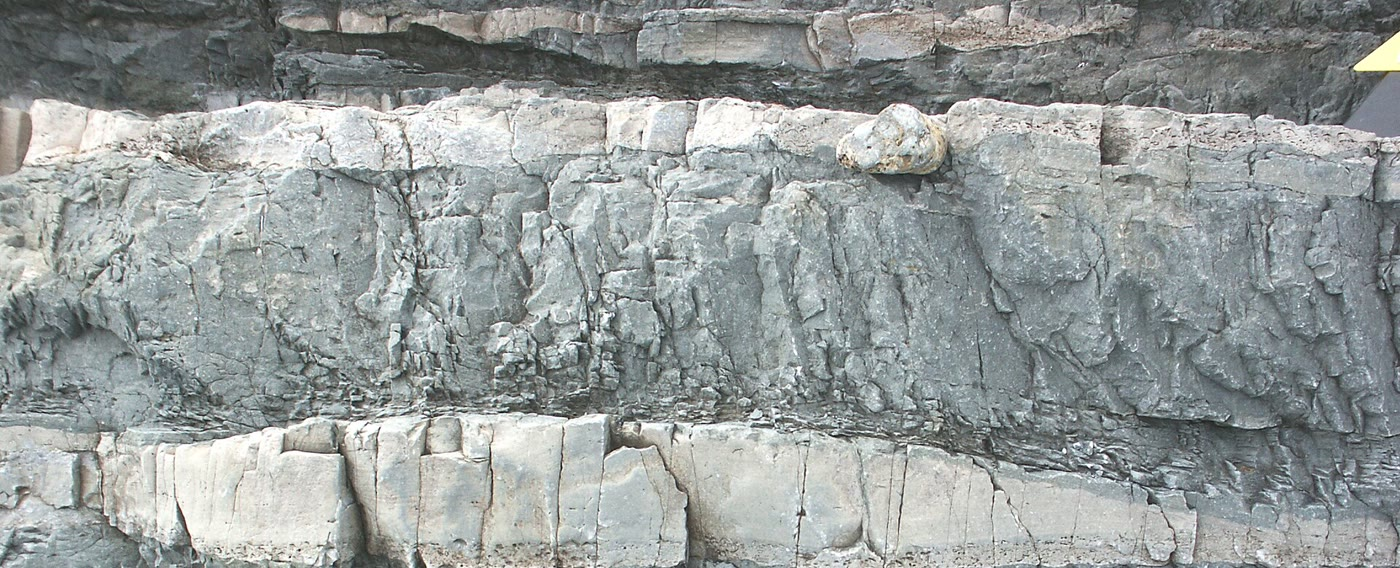
\includegraphics[width=\linewidth]{images/book5/b3-hummocky-cross-stratification.jpg}

{\scriptsize \omterm{def:b3:facies-models:hcs}{Hummocky kruisgelaagdheid} in de Arisaig-formatie
(Siluur), nabij Arisaig, Nova Scotia. Foto Michael C. Rygel, CC BY-SA 3.0
(bijgesneden).}
\end{minipage}
\end{inthefield}
% ledger: photo:b3-hcs

Waar getijden domineren, verandert de faciës: vloed- en ebstromen bouwen
kruislagen op die in tegengestelde richtingen wijzen, modderlagen bezinken bij elk stilwater, en
de dikte van de pakketten tussen de modderlagen neemt toe en af met de cyclus van
springtij en doodtij. Getijdegeulen, -platen en zandruggen
hebben hun eigen modellen, op dezelfde manier opgebouwd.

\section{Diepe zee}\label{sec:b3:facies-models:deep}

Een troebelingsstroom die vertraagt, zet zijn lading af in de volgorde van bezinking:
de grofste korrels eerst, de fijnste als laatste. Een volledige turbidietlaag toont
deze volgorde in vijf onderdelen.

\begin{definition}[Bouma-sequentie]\label{def:b3:facies-models:bouma}
De \emph{Bouma-sequentie}\index{Bouma-sequentie} is de ideale opeenvolging van
onderdelen in een turbidietlaag, van onder naar boven: Ta, massief of gegradeerd zand op
een erosief grensvlak met stroomgroeven en gereedschapssporen; Tb, parallel gelamineerd zand; Tc,
rimpelkruislaminatie en geplooid fijn zand; Td, parallel gelamineerd silt;
Te, modder, deels uit de troebelingsstroom en deels uit het langzame bezinken
tussen de stromingen.
\end{definition}

Weinig lagen tonen alle vijf: dicht bij de bron is de stroom snel en laat hij dikke
Ta-onderdelen achter, waarvan de bovenste door de volgende stroming worden geërodeerd; ver ervandaan alleen
de fijnere onderdelen, Tc tot en met Te, aan. De opeenvolging legt zo het
afnemen van één stroming vast, en de verandering van de lagen langs de waaier het
afnemen van de stromingen met de afstand.

\begin{definition}[Onderzeese waaier]\label{def:b3:facies-models:fan}
Een \emph{onderzeese waaier}\index{onderzeese waaier} is een kegel van sediment aan de voet
van een continentale helling, gevoed door een canyon: een bovenste waaier met een hoofdgeul
tussen oeverwallen, een middelste waaier van vertakkende geulen die uitmonden in zandloben,
en een onderste waaier van dunne turbidieten die overgaan in modder van de bekkenbodem.
\end{definition}

Langs de marge herwerken diepe stromingen, aangedreven door de circulatie van de oceaan, het
fijne sediment van de helling tot contourieten, heuvels en drifts van
door organismen omgewoelde silt en modder die langs de contourlijnen groeien in plaats van de
helling af.

\begin{omfigure}
\begin{tikzpicture}[font=\scriptsize, x=1cm, y=1cm]
% (a) Bouma log
\begin{scope}
\fill[yellow!45] (0,0) -- (1.6,0) -- (1.6,1.2) -- (0,1.2) -- cycle;
\fill[yellow!35] (0,1.2) rectangle (1.3,1.8);
\fill[yellow!25] (0,1.8) rectangle (1.0,2.4);
\fill[black!12] (0,2.4) rectangle (0.7,2.8);
\fill[black!25] (0,2.8) rectangle (0.4,3.3);
\draw (0,0) -- (1.6,0) -- (1.6,1.2) -- (1.3,1.2) -- (1.3,1.8) -- (1.0,1.8) -- (1.0,2.4) -- (0.7,2.4) -- (0.7,2.8) -- (0.4,2.8) -- (0.4,3.3) -- (0,3.3) -- cycle;
\draw[decorate, decoration={snake, amplitude=0.5mm, segment length=2mm}] (0,0) -- (1.6,0);
\foreach \y in {1.35,1.5,1.65} {\draw[black!60] (0.05,\y) -- (1.25,\y);}
\foreach \x in {0.15,0.45,0.75} {\draw[black!60] (\x,1.95) .. controls (\x+0.08,2.1) .. (\x+0.2,1.95);}
\foreach \y in {2.5,2.6,2.7} {\draw[black!60] (0.05,\y) -- (0.65,\y);}
\foreach \y/\t in {0.6/Ta, 1.5/Tb, 2.1/Tc, 2.6/Td, 3.05/Te} {\node[anchor=west] at (1.9,\y) {\t};}
\node[anchor=west, align=left, font=\tiny] at (2.4,0.6) {gegradeerd of massief zand,\\ erosief grensvlak};
\node[anchor=west, font=\tiny] at (2.4,1.5) {parallelle laminae};
\node[anchor=west, font=\tiny] at (2.4,2.1) {rimpels, geplooide laminae};
\node[anchor=west, font=\tiny] at (2.4,2.6) {gelamineerd silt};
\node[anchor=west, font=\tiny] at (2.4,3.05) {modder};
\node[anchor=north] at (1.6,-0.15) {(a) een turbidietlaag};
\end{scope}
% (b) fan plan
\begin{scope}[xshift=8.2cm, yshift=0.2cm]
\fill[black!8] (-1.0,-0.2) rectangle (5.6,3.1);
\fill[yellow!20] (0.3,2.9) .. controls (1.6,2.6) and (4.9,2.0) .. (5.2,0.9) .. controls (4.6,-0.1) and (1.2,0.1) .. (0.3,1.6) -- cycle;
\fill[yellow!45] (1.9,1.9) ellipse (0.55 and 0.3);
\fill[yellow!45] (2.6,1.0) ellipse (0.55 and 0.3);
\fill[yellow!45] (3.4,1.75) ellipse (0.5 and 0.28);
\draw[omDef, line width=1.4pt] (-0.9,3.0) .. controls (-0.3,2.8) and (0.4,2.6) .. (1.0,2.2);
\draw[omDef, line width=0.8pt] (1.0,2.2) -- (1.6,1.95);
\draw[omDef, line width=0.8pt] (1.0,2.2) -- (2.3,1.15);
\draw[omDef, line width=0.8pt] (1.0,2.2) .. controls (2.0,2.4) .. (3.1,1.85);
\node[anchor=south west] at (-0.95,3.0) {canyon};
\node[anchor=east] at (0.55,2.0) {oeverwallen};
\node[align=center, font=\tiny] at (2.6,1.0) {zandlob};
\node at (4.4,0.7) {onderste waaier};
\node[black!60] at (4.9,2.85) {bekkenbodem};
\node[anchor=north] at (2.3,-0.25) {(b) een onderzeese waaier in plan};
\end{scope}
\end{tikzpicture}

\par\smallskip{\small (a) De \omterm{def:b3:facies-models:bouma}{Bouma-sequentie} van een volledige turbidietlaag,
weergegeven als korrelgroottelog (breedte betekent grover), met zijn vijf divisies. (b)
Een \omterm{def:b3:facies-models:fan}{onderzeese waaier} in plan: een canyon voedt een geul tussen oeverwallen, die
splitst in verdelende geulen die eindigen in zandlobben; dunne turbidieten
verspreiden zich over de onderste waaier.}\label{fig:b3:facies-models:deep}
\end{omfigure}

\section{Carbonaatplatforms}\label{sec:b3:facies-models:carbonates}

Carbonaatsediment ontstaat waar het ligt, door organismen in warm, helder,
ondiep water, en de facies volgen het profiel van het platform dat de
carbonaatfabriek voor zichzelf bouwt.

\begin{definition}[Carbonaatramp en omzoomd plat]\label{def:b3:facies-models:ramp}
Een \emph{carbonaatramp}\index{carbonaatramp} is een platform waarvan de bodem
zacht en gelijkmatig van de kustlijn naar het bekken helt, zonder breuk:
zijn faciesgordels, van getijdenvlakten en strandbarrièrezanden tot korrels uit ondiepe banken,
bioklastisch zand en kalkmodder van de open zee, zijn breed en gaan geleidelijk in
elkaar over, gesorteerd door de golfenergie die met de diepte afneemt. Een \emph{omzoomd
plat}\index{omzoomd plat} is een platform met een vlakke top en een duidelijke knik
in de helling aan de rand, waar riffen en zandbanken een rand opbouwen die
een lagune achter zich beschermt; voorbij de rand levert een steile helling blokken en korrels af aan
het bekken.
\end{definition}

\begin{omfigure}
\begin{tikzpicture}[font=\scriptsize, x=1cm, y=1cm]
\begin{scope}
\fill[omSea!60] (0,1.6) -- (6.4,1.6) -- (6.4,0.3) -- cycle;
\fill[black!10] (0,1.6) -- (6.4,0.3) -- (6.4,0) -- (0,0) -- cycle;
\draw[thick] (0,1.7) -- (0.3,1.6) -- (6.4,0.3);
\draw[omDef] (0,1.6) -- (6.4,1.6);
\node[anchor=south] at (0.6,1.65) {getijdenvlakte};
\node[rotate=-12, font=\tiny] at (1.5,1.08) {korrels uit ondiepe banken};
\node[rotate=-12, font=\tiny] at (3.4,0.66) {bioklastisch zand};
\node[rotate=-12, font=\tiny] at (5.3,0.26) {kalkmodder};
\node[anchor=north] at (3.2,-0.1) {(a) ramp: een gelijkmatige helling, geleidelijke gordels};
\end{scope}
\begin{scope}[xshift=7.2cm]
\fill[omSea!60] (0,1.6) -- (6.4,1.6) -- (6.4,0.2) -- (4.4,0.3) -- (3.6,1.55) -- (3.2,1.6) -- (0.3,1.6) -- cycle;
\fill[omSea!60] (0.3,1.6) -- (3.2,1.6) -- (3.0,1.35) -- (0.6,1.35) -- cycle;
\fill[black!10] (0,1.7) -- (0.3,1.6) -- (0.6,1.35) -- (3.0,1.35) -- (3.2,1.6) -- (3.6,1.55) -- (4.4,0.3) -- (6.4,0.2) -- (6.4,0) -- (0,0) -- cycle;
\draw[thick] (0,1.7) -- (0.3,1.6) -- (0.6,1.35) -- (3.0,1.35) -- (3.2,1.6) -- (3.6,1.55) -- (4.4,0.3) -- (6.4,0.2);
\fill[orange!50] (3.05,1.4) -- (3.2,1.6) -- (3.55,1.56) -- (3.6,1.4) -- cycle;
\draw[omDef] (0,1.6) -- (6.4,1.6);
\node at (1.8,1.12) {lagune};
\node[anchor=south] at (3.35,1.65) {rifrand};
\node[anchor=west] at (4.2,0.95) {steile helling};
\node at (5.5,0.6) {bekken};
\node[anchor=north] at (3.2,-0.1) {(b) omzoomd plat: een rand, een lagune, een helling};
\end{scope}
\end{tikzpicture}

\par\smallskip{\small Carbonaatplatformprofielen (schematisch, verticale schaal
sterk overdreven). (a) Een ramp: gordels gesorteerd door golfenergie langs een
gelijkmatige helling. (b) Een \omterm{def:b3:facies-models:ramp}{omzoomd plat}: een rand van riffen en zandbanken bij de knik
in de helling beschermt een lagune met kalkmodder; de helling daarachter ontvangt blokken en korrels
die van de rand afkomen.}\label{fig:b3:facies-models:platforms}
\end{omfigure}

Op een vlakke platformtop overstroomt een kleine stijging van het relatieve zeeniveau de
getijdenvlakten, en de fabriek, die het snelst werkt in het ondiepste water, vult de
ruimte binnen korte tijd weer op tot het zeeniveau. Het resultaat is een stapel
peritidale cycli van een meter of enkele meters dik, elk een opwaarts ondieper wordende
\omterm{def:b3:sequence-stratigraphy:parasequence}{parasequentie} van subtidale modder tot een getijdenvlakte met uitdrogingsscheuren of
microbiële matten, afgesloten door het volgende \omterm{def:b3:sequence-stratigraphy:parasequence}{overstromingsvlak}.

\section{Boorkernen en boorgatlogs}\label{sec:b3:facies-models:logs}

Het grootste deel van het gesteente onder sedimentaire bekkens is bekend uit boorgaten. Enkele
worden gekernd, en hun kernen worden laag voor laag beschreven, zoals men een klif zou beschrijven; bijna alle
worden gelogd.

\begin{definition}[Boorgatlogs]\label{def:b3:facies-models:wireline}
Een \emph{boorgatlog}\index{boorgatlog} is een continue registratie van een
fysische eigenschap van de gesteenten als functie van de diepte, gemeten door een sonde die aan
een kabel in een boorgat wordt neergelaten. De \emph{gammalog}\index{gammalog}
registreert de natuurlijke gammastraling van het gesteente, in API-eenheden: hoog in
schalie, waarvan de kleien kalium, thorium en uranium bevatten, laag in zuiver
kwartszand en in kalksteen. De \emph{dichtheidslog}\index{dichtheidslog}
registreert de volumedichtheid uit de verstrooiing van gammastralen die door een
bron op de sonde worden uitgezonden. De \emph{sonische log}\index{sonische log} registreert de
intervallooptijd van een compressiegolf, in microseconden per voet. De
\emph{neutronenlog}\index{neutronenlog} registreert het afremmen van neutronen door
waterstof, en dus het water dat in de poriën en in de kleien zit.
\end{definition}
% ledger: keys:gamma, keys:density-porosity, keys:sonic

De API-gammastralingseenheid is gedefinieerd in een kalibratieput: een tweehonderdste van
het verschil tussen een zone met verwaarloosbare radioactiviteit en een zone met
de radio-isotopen van een gemiddelde schalie op ongeveer het dubbele van zijn concentratie. Kolen,
kalksteen en dolomiet zijn meestal minder radioactief dan schalie; kwartszandsteen
is laag, een arkose rijk aan kaliumveldspaat hoger; elk gesteente kan radioactief worden
gemaakt door uranium dat door grondwater wordt aangevoerd.
% ledger: keys:gamma

\begin{proposition}[Porositeit uit dichtheid en looptijd]\label{prop:b3:facies-models:porosity}
Een gesteente met porositeit $\phi$, met korrels van dichtheid $\rho_{\mathrm{ma}}$ en
poriën gevuld met een vloeistof van dichtheid $\rho_f$, heeft de volumedichtheid
$\rho_b = (1 - \phi)\rho_{\mathrm{ma}} + \phi\rho_f$, zodat
\[
\phi = \frac{\rho_{\mathrm{ma}} - \rho_b}{\rho_{\mathrm{ma}} - \rho_f}.
\]
Als een compressiegolf de korrels en de vloeistof achter elkaar doorkruist, over
lengten evenredig met $1 - \phi$ en $\phi$, dan is de looptijd
$\Delta t = (1 - \phi)\Delta t_{\mathrm{ma}} + \phi\Delta t_f$ (de
tijdgemiddelde vergelijking), en $\phi = (\Delta t - \Delta
t_{\mathrm{ma}})/(\Delta t_f - \Delta t_{\mathrm{ma}})$.
\end{proposition}

\begin{proof}
Een eenheidsvolume gesteente bevat een volume $1 - \phi$ aan korrels en $\phi$ aan
vloeistof; de massa is $(1 - \phi)\rho_{\mathrm{ma}} + \phi\rho_f$, waaruit
$\phi$ wordt opgelost. Voor de golf kruist een weg van eenheidslengte $1 - \phi$ aan
korrels en $\phi$ aan vloeistof, en de tijden tellen op.
\end{proof}

Korreldichtheden zijn \qty{2.65}{g/cm^3} voor kwarts en \qty{2.71}{g/cm^3} voor
kalksteen; het porievocht is \qty{1.0}{g/cm^3} wanneer het zoet is en oploopt tot
\qty{1.1}{g/cm^3} als pekel. Looptijden variëren van 42 tot
\qty{48}{\micro\second/ft} in dolomiet, 48 tot 53 in kalksteen, 53 voor een
verkitte zandsteen, en 189 in pekel. De dichtheidsvergelijking is exact voor
een bekende matrix; de tijdgemiddelde vergelijking is een empirische regel die
het best werkt in verkitte gesteenten met intergranulaire poriën. Schalie voldoet aan geen van beide:
kleien hebben hun eigen dichtheden en houden gebonden water vast.
% ledger: keys:density-porosity, keys:sonic

\begin{definition}[Net-to-gross-verhouding]\label{def:b3:facies-models:ntg}
De \emph{net-to-gross-verhouding}\index{net-to-gross-verhouding} van een interval is de
dikte van zijn reservoirkwaliteit gesteente, meestal zand dat op het \omterm{def:b3:facies-models:wireline}{gammalog} wordt
afgelezen onder een afkapwaarde, gedeeld door de totale dikte van het interval.
\end{definition}

De vorm van de gammacurve door een zandlichaam is een faciesinstrument.
Een \emph{klok}, schoon aan de basis en opwaarts kleiiger, is een \omterm{def:b3:facies-models:association}{opwaarts fijner wordende
opeenvolging}, zoals in een \omterm{def:b3:facies-models:rivers}{kronkelwaard} of een geulvulling; een \emph{trechter}, kleiig aan
de basis en schoon aan de top, een \omterm{def:b3:facies-models:association}{opwaarts grover wordende opeenvolging}, zoals in een
prograderende \omterm{def:b3:facies-models:shoreface}{onderwateroever} of deltafront; een \emph{cilinder}, overal schoon met
scherpe grenzen, een gestapelde zandlaag van een \omterm{def:b3:facies-models:rivers}{verwilderde rivier}, een eolische duin of een
carbonaatbank. De vormen zijn aanwijzingen, geen bewijzen: een kern, of ten minste de
naburige logs, moet ze bevestigen.

\begin{omfigure}
\begin{tikzpicture}
\begin{groupplot}[group style={group size=3 by 1, horizontal sep=0.2cm,
    y descriptions at=edge left},
  omrecord, y dir=reverse, ymin=700, ymax=1200, width=0.28\linewidth,
  height=0.62\linewidth, ytick={700,800,900,1000,1100,1200},
  tick label style={font=\scriptsize}, label style={font=\small},
  xlabel style={font=\small}]
\nextgroupplot[xlabel={GR (API)}, ylabel={diepte (m)}, xmin=0, xmax=150,
  xtick={0,50,100,150}]
\addplot[black!60, densely dashed, forget plot] coordinates {(60,1046) (60,1166)};
% computed in figdata/bachelor-3/well_logs.py
\addplot[omDef, thin] table[x=gr, y=depth] {figdata/out/bachelor-3-well_logs-logs.dat};
\node[font=\scriptsize, anchor=west] at (axis cs:2,730) {krijt};
\node[font=\scriptsize, anchor=west] at (axis cs:2,816) {schalie};
\node[font=\scriptsize, anchor=west] at (axis cs:28,956) {kalksteen};
\node[font=\scriptsize, anchor=west] at (axis cs:28,1030) {zandsteen};
\node[font=\scriptsize, anchor=west] at (axis cs:2,1185) {schist};
\nextgroupplot[xlabel={$\rho_b$ (\unit{g/cm^3})}, xmin=1.9, xmax=2.9,
  xtick={2.0,2.4,2.8}, xticklabels={2.0,2.4,2.8}]
\addplot[red!70!black, thin] table[x=rhob, y=depth] {figdata/out/bachelor-3-well_logs-logs.dat};
\nextgroupplot[xlabel={$\Delta t$ (\unit{\micro\second/ft})}, xmin=40, xmax=140,
  x dir=reverse, xtick={40,80,120}]
\addplot[green!40!black, thin] table[x=dt, y=depth] {figdata/out/bachelor-3-well_logs-logs.dat};
\end{groupplot}
\begin{axis}[at={(group c3r1.south east)}, xshift=1.35cm, anchor=south west,
  omrecord, y dir=reverse, ymin=1040, ymax=1172, width=0.28\linewidth,
  height=0.62\linewidth, xmin=0, xmax=120, xtick={0,60,120},
  ytick={1040,1060,1080,1100,1120,1140,1160}, ylabel={diepte (m)},
  xlabel={GR (API), zandsteen}, tick label style={font=\scriptsize},
  label style={font=\small}]
\addplot[black!60, densely dashed, forget plot] coordinates {(60,1046) (60,1166)};
\addplot[omDef, semithick] table[x=gr, y=depth] {figdata/out/bachelor-3-well_logs-sand.dat};
\end{axis}
\end{tikzpicture}

\par\smallskip{\small Synthetische logs van de put Varden-2 van \qty{700}{m}
tot het basement: gammastraling (de gestreepte lijn is de zandafkapwaarde van
\qty{60}{API} in het zandsteen), volumedichtheid en sonische looptijd (tijd
toenemend naar links, zoals logs worden getekend); rechts de gammastraling van
het zandsteen vergroot. Het krijt wordt dichter met de diepte;
de schalie reageert warm, traag en met een tussenliggende dichtheid; de kalksteen is koud,
dicht en snel; het zandsteen is een stapel geulvullingen, elk met een schone basis
die opwaarts overgaat in modder: klokvormen.}\label{fig:b3:facies-models:logs}
\end{omfigure}
% ledger: keys:gamma, keys:density-porosity, keys:sonic

\begin{inthelab}[Een kern beschrijven]
\begin{minipage}[t]{0.5\linewidth}\vspace{0pt}
In een kernopslag liggen de kernen van een put in bakken, overlangs gespleten,
in de volgorde van hun diepte. Een sedimentoloog beschrijft de
kern laag voor laag op een logformulier: korrelgrootte met een handlens en een vergelijkingstabel,
structuren, grenzen, fossielen, sporen van gangen en wortels, de kleur
van de modder. De beschrijving wordt daarna naast de \omterm{def:b3:facies-models:wireline}{boorgatlogs} van
dezelfde dieptes gelegd, waarmee de logvormen aan het gesteente worden geijkt en de
naburige putten zonder kern kunnen worden gelezen.
\end{minipage}\hfill
\begin{minipage}[t]{0.46\linewidth}\vspace{0pt}
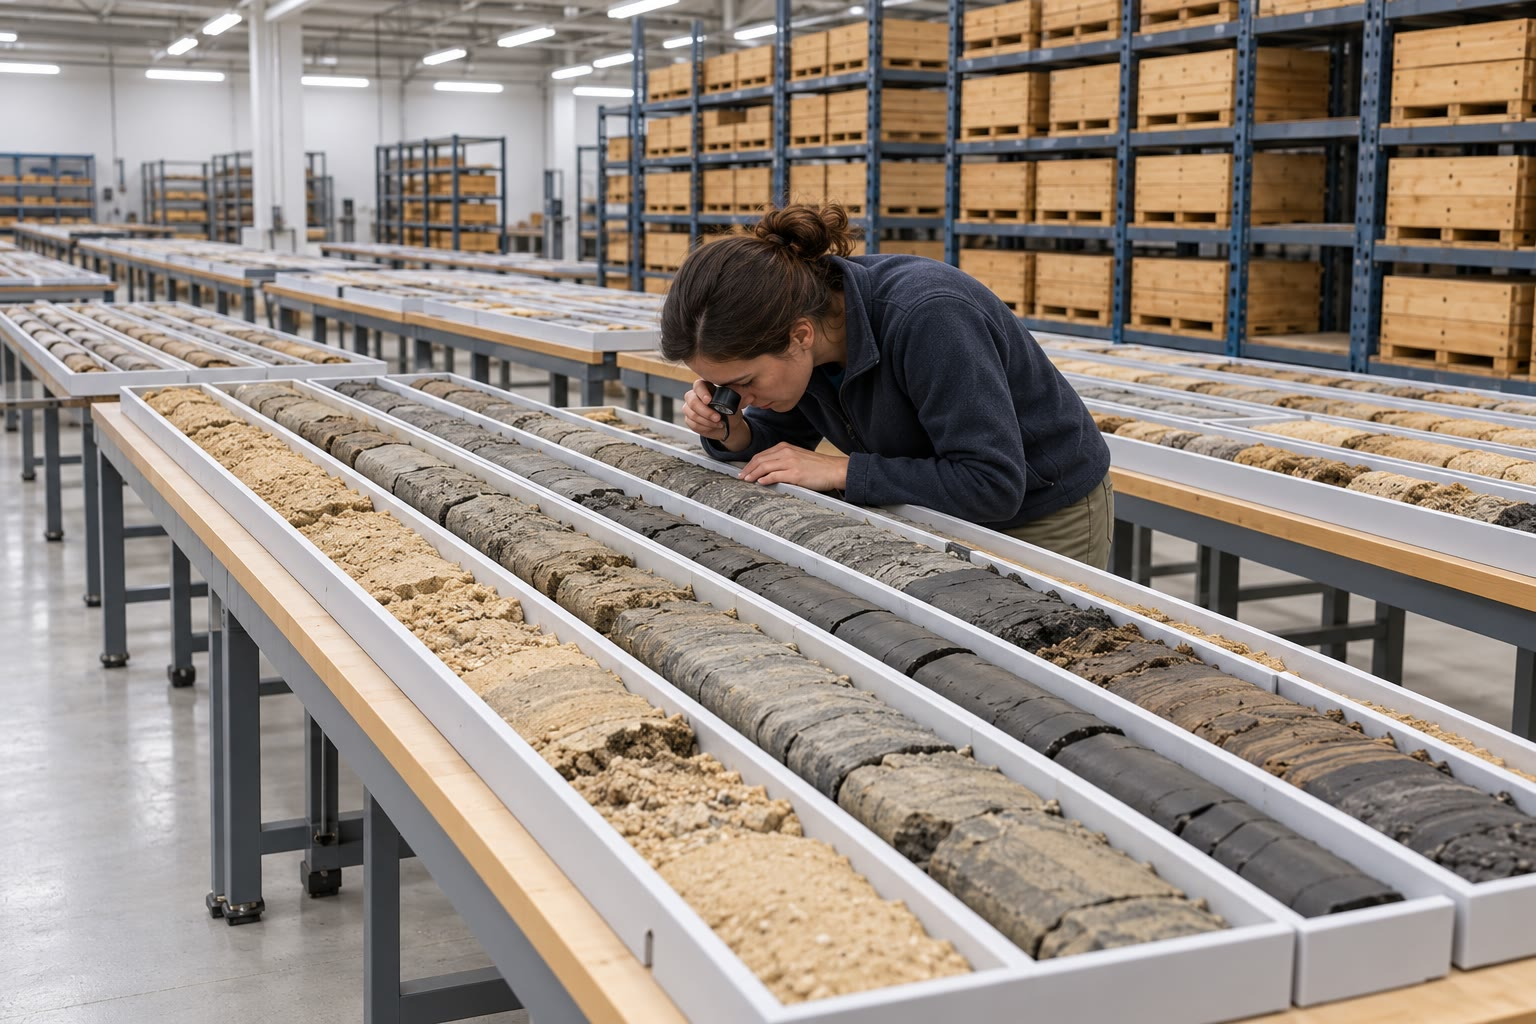
\includegraphics[width=\linewidth]{images/book5/ai/b3-core-store.jpg}

{\scriptsize Een kernopslag: gespleten kernen van zand en modder in bakken, een geoloog
met een handlens. Door AI gegenereerde illustratie.}
\end{minipage}
\end{inthelab}

\section{Oefeningen}

\begin{exercise}[$\star$]\label{exo:b3:facies-models:1}
Een kern toont van onder naar boven: offshore modder, afwisselend gelaagde modder en fijn zand,
onderwateroeverzand, strandzand, dan steenkool met wortels. Gebruik de wet van Walther en geef
de volgorde van de milieus langs de kust op dat moment en de richting
waarin de kustlijn bewoog. Wat zou een transgressie hebben achtergelaten?
\end{exercise}

\begin{exercise}[$\star$]\label{exo:b3:facies-models:2}
Drie zandlichamen tonen gammastralingsvormen: (a) een klok van \qty{8}{m} dik met een
scherpe basis; (b) een trechter van \qty{20}{m} dik; (c) een cilinder van \qty{30}{m}
dik met een scherpe top en basis. Stel voor elk een milieu voor, en de
waarneming in een kern die dat zou bevestigen.
\end{exercise}

\begin{exercise}[$\star$]\label{exo:b3:facies-models:3}
Een zandsteen geeft $\rho_b = \qty{2.40}{g/cm^3}$. Bereken de porositeit met
een kwartsmatrix en zoetwater, en daarna met pekel van \qty{1.1}{g/cm^3}.
\end{exercise}
% ledger: keys:density-porosity

\begin{exercise}[$\star$]\label{exo:b3:facies-models:4}
Golven met een modale golflengte van \qty{75}{m} en \qty{110}{m} (de beschutte en
de open zee van de boeienstudie). Schat de diepte waarop elk
\qty{4}{\percent} van zijn oppervlaktebeweging behoudt, en de fractie
die op een diepte van \qty{20}{m} overblijft.
\end{exercise}
% ledger: losspeters10:wavebase

\begin{exercise}[$\star\star$]\label{exo:b3:facies-models:5}
Een kalksteen geeft $\Delta t = \qty{60}{\micro\second/ft}$. Bereken de
porositeit met de tijdgemiddelde vergelijking voor een matrix van 47.6 en van
\qty{52.6}{\micro\second/ft} en pekel bij \qty{189}{\micro\second/ft}. Wat
leert het verschil?
\end{exercise}
% ledger: keys:sonic

\begin{exercise}[$\star\star$]\label{exo:b3:facies-models:6}
Een interval van \qty{40}{m} bevat zandlagen van 6.0, 3.5, 8.0 en \qty{2.5}{m}
onder de afkapwaarde, de rest is slib. Bereken de \omterm{def:b3:facies-models:ntg}{net-to-gross-verhouding}. Met
een porositeit van \qty{22}{\percent} in het zand, hoeveel porievolume bevat een
vierkante kilometer van het interval?
\end{exercise}

\begin{exercise}[$\star\star$]\label{exo:b3:facies-models:7}
Een turbidietlaag nabij de monding van een canyon bestaat uit \qty{1.2}{m} massief zand
(Ta) dat aan de top is geërodeerd door de volgende laag; \qty{30}{km} verder de waaier af ligt een laag van
dezelfde troebelingsstroom: \qty{8}{cm} rimpelgelaagd fijn zand en silt onder
\qty{3}{cm} slib. Benoem de divisies van elk en verklaar de verandering.
\end{exercise}

\begin{exercise}[$\star\star$]\label{exo:b3:facies-models:8}
Een \omterm{def:b3:facies-models:association}{opwaarts fijner wordende opeenvolging} van \qty{9}{m} dik heeft een scherpe basis met
kiezels, kruisgelaagd zand, rimpelgelaagd fijn zand en slib met wortelsporen. Interpreteer
haar en schat de diepte van de geul die haar heeft gevormd. Kan de wet van Walther
over haar basis worden toegepast? Waarom?
\end{exercise}

\begin{exercise}[$\star\star$]\label{exo:b3:facies-models:9}
Een platformbodem zakt \qty{60}{m} over \qty{40}{km}; een andere houdt een
diepte van \qty{5}{m} over \qty{30}{km} aan en zakt daarna \qty{300}{m} over
\qty{1.5}{km}. Bereken beide hellingen, benoem elk platform en het faciës dat
aan de rand van het tweede wordt verwacht.
\end{exercise}

\begin{exercise}[$\star\star\star$]\label{exo:b3:facies-models:10}
Een kustlijn progradeert met een snelheid $v$, terwijl het relatieve zeeniveau stijgt met
een snelheid $A$, en de onderwateroevergordel is $w$ breed. Toon aan dat het
onderwateroeverzand in de verticale opeenvolging $h = wA/v$ dik is. Bereken het voor
$w = \qty{2}{km}$, $A = \qty{0.2}{m/kyr}$ en $v = \qty{20}{m/kyr}$, en zeg wat er gebeurt
wanneer $A = 0$. Vergelijk met de propositie over het \omterm{def:b3:sequence-stratigraphy:trajectory}{kustlijntraject} in
Hoofdstuk~\ref{ch:b3:sequence-stratigraphy}.
\end{exercise}

\begin{exercise}[$\star\star\star$]\label{exo:b3:facies-models:11}
Een zandsteen geeft $\rho_b = \qty{2.30}{g/cm^3}$ en $\Delta t =
\qty{86}{\micro\second/ft}$. Bereken de porositeit uit elk log met een
kwartszandsteenmatrix (2.65, \qty{52.6}{\micro\second/ft}) en pekel (1.0 voor de
dichtheid, \qty{189}{\micro\second/ft}). Als de sonische porositeit juist is, welke
korreldichtheid impliceert het \omterm{def:b3:facies-models:wireline}{dichtheidslog} dan, en wat kan het cement zijn?
\end{exercise}
% ledger: keys:density-porosity, keys:sonic

\begin{exercise}[$\star\star\star$]\label{exo:b3:facies-models:12}
In een boorkern ligt zwart offshore-slib direct op steenkool met wortelsporen, met een
dunne laag schelpenpuin op het contact. Verklaar waarom de wet van Walther hier niet
geldt, welk oppervlak het is, en hoeveel van de kustsuccessie mogelijk ontbreekt als
golven de bodem hebben weggeslagen tot een \omterm{def:b3:facies-models:shoreface}{golfbasis bij mooi weer} van ongeveer
\qty{10}{m} toen de kustlijn passeerde.
\end{exercise}

\section{Probleem: Varden-2, een boring door de bedekking}

\begin{problem}[{Weekendprobleem --- de logs, porositeit, faciës en netto
zand van een verzonnen boring in de Varden-synclinale}]
\label{pb:b3:facies-models:1}
De boring Varden-2 wordt geboord in de synclinale van de Varden-heuvels, op
(7500, 7000) op het rooster van de regio, vanaf een maaiveldhoogte van
\qty{441.0}{m}, tot een totale diepte van \qty{1200}{m}. Haar logs zijn getekend in de
figuur van de vorige paragraaf. Gebruik korreldichtheden van 2.65 (kwarts) en
\qty{2.71}{g/cm^3} (calciet), een porewater van \qty{1.0}{g/cm^3}, matrixdoorlooptijden
van 52.6 (zandsteen) en \qty{47.6}{\micro\second/ft}
(kalksteen), en \qty{189}{\micro\second/ft} voor het water.

\medskip\noindent\textbf{Deel I --- De logs aflezen.}
\begin{enumerate}
\item De gammastraling springt van 12 naar \qty{110}{API} op \qty{766}{m}, daalt
  naar 18 op \qty{866}{m}, wordt onregelmatig vanaf \qty{1046}{m} en blijft constant op
  \qty{85}{API} vanaf \qty{1166}{m}. Benoem de eenheden die zijn aangetroffen, aan de hand van hun logs.
\item Bereken de dikte van elke eenheid van de bedekking en de hoogte van
  de basis van de bedekking.
\item Het krijt geeft \qty{2.03}{g/cm^3} nabij het oppervlak en
  \qty{2.36}{g/cm^3} op \qty{750}{m}. Bereken de porositeit op beide diepten.
  Wat gebeurt er met het krijt naarmate de diepte toeneemt?
\item Waarom wordt aan de schalie geen porositeit toegekend op grond van haar dichtheid?
\item Het schist geeft \qty{2.75}{g/cm^3} en \qty{50}{\micro\second/ft}.
  Wat vertelt het snelle, dichte, niet-poreuze grondgebergte de boormeester?
\end{enumerate}

\medskip\noindent\textbf{Deel II --- Porositeit.}
\begin{enumerate}[resume]
\item Het kalksteen geeft \qty{2.573}{g/cm^3}: bereken de dichtheidsporositeit.
\item Het geeft \qty{58.9}{\micro\second/ft}: bereken de sonische porositeit en
  vergelijk.
\item Het schone zand van de geulvullingen geeft \qty{2.32}{g/cm^3}: bereken
  de porositeit.
\item Controleer dit met de doorlooptijd, \qty{79.9}{\micro\second/ft}.
\item Als het porewater een pekel van \qty{1.1}{g/cm^3} zou zijn, met hoeveel zou
  de dichtheidsporositeit van het zand dan veranderen?
\item Welke eenheid zou de betere watervoerende laag of het betere reservoir vormen, en welke
  de afdichting erboven vormt?
\end{enumerate}

\medskip\noindent\textbf{Deel III --- Facies.} Een kern die van 1108 tot
\qty{1124}{m} is geboord, toont van onderaf: een erosievlak met modderknollen en
kiezels; \qty{10.4}{m} kruisgelaagd middelgroot zand; \qty{3.2}{m} gerimpeld
fijn zand dat overgaat in silt; \qty{2.4}{m} roodbruine klei met wortelsporen.
\begin{enumerate}[resume]
\item Teken de verwachte gammalogvorm over het geboorde interval.
\item Benoem de opeenvolging en het afzettingsmilieu van elk deel.
\item Beschrijf met de wet van Walther de milieus die naast elkaar liggen.
\item Schat de diepte van de geul.
\item Het zandsteen bevat elf van zulke eenheden, elk op een scherpe basis. Wat zegt
  de stapeling over de rivier en haar overstromingsvlakte?
\item Kan de wet van Walther worden gebruikt om van de ene eenheid naar de volgende? Waarom?
\end{enumerate}

\medskip\noindent\textbf{Deel IV --- Netto zand.} De elf geulvullingen,
vanaf de basis van het zandsteen, zijn 14, 9, 12, 7, 16, 10, 13, 8, 11, 12 en
\qty{8}{m} dik. Elk begint met schoon zand (\qty{30}{API}) over een deel
van hun dikte van 0.60, 0.45, 0.55, 0.30, 0.65, 0.40, 0.55, 0.35, 0.50,
0.45 en 0.30, en wordt dan fijner naar boven over een deel van 0.25, 0.30, 0.25, 0.40,
0.20, 0.30, 0.25, 0.35, 0.25, 0.30 en 0.35, waarbij de gammastraling lineair stijgt tot
\qty{105}{API}, en eindigt in modder.
\begin{enumerate}[resume]
\item Welk deel van elk fijnend interval ligt onder de
  afkapwaarde van \qty{60}{API}?
\item Bereken het netto zand van de onderste eenheid en van de dikste.
\item Bereken het totaal van het schone zand en het totaal van de fijnende intervallen van het
  zandsteen.
\item Bereken de \omterm{def:b3:facies-models:ntg}{net-to-gross-verhouding}.
\item Hoe zou het netto zand veranderen bij een afkapwaarde van 45 of van
  \qty{75}{API}?
\item Bereken met de zandporositeit uit vraag 8 het porievolume van het
  netto zand onder een vierkante kilometer.
\item Geef de netto-zanddikte van het Trias-zandsteen bij Varden-2.
\end{enumerate}
\end{problem}
% ledger: keys:density-porosity, keys:sonic, keys:gamma
